\documentclass[10pt]{article}
\usepackage[spanish]{babel}
\usepackage{graphicx}
\usepackage{tabularx} % para width table
\usepackage[left=1.5cm,top=2.4cm,right=2.1cm,bottom=3cm,bindingoffset=0.5cm]{geometry} % original[22 iz,24 arri]
\usepackage{multirow}
\graphicspath{{img/}{img2/}}
\usepackage{url}
\usepackage[document]{ragged2e}

\usepackage{mathtools}
\usepackage{amsmath}
\usepackage{mathrsfs} 
%\usepackage{natbib}
\usepackage{float}


\begin{document}
	
	
	\centering
	\begin{tabular}{ |	p{30 mm}|	p{61 mm}	|	p{33mm}	| p{43mm}	| } 
		\hline
		
		
		\multirow{4}{30mm}{\centering 
\includegraphics[scale=0.22]{logo}} &
		\multirow{4}{61mm}{\centering \textbf{ \textbf{Manual de prácticas del Laboratorio de Análisis de Sistemas y Señales}}}    & Código: & MADO-76 \\
		\cline{3-4}
		& &  Versión & 01 \\
		\cline{3-4}
		& & Página: & 63/97 \\ \cline{3-4}
		& & Sección ISO: & 8.3 \\ \cline{3-4}
		& & Fecha de emisión: & 28 de frebrero 2019 \\
		\hline
	\end{tabular}
\begin{tabular}{ |	c |	c	| } 
	
	\multirow{2}{65mm}{ \centering Facultad de ingeniería} &
	\multirow{2}{111mm}{\centering \textbf{ Area/Departamento: \\ Laboratorio de control y robótica}}   \\
	& \\ \hline
\end{tabular}
\begin{tabular}{|p{180mm}|}
	\multirow{1}{180mm}{ \centering La impresion de este documento es una copia no controlada }  \\ \hline \end{tabular} \\

\vspace{1cm}


{\centering \LARGE Práctica N◦4 Fundamentos de modelado de sistemas físicos}

\vspace{1.5cm}

\begin{figure}[!h]
	\centering
	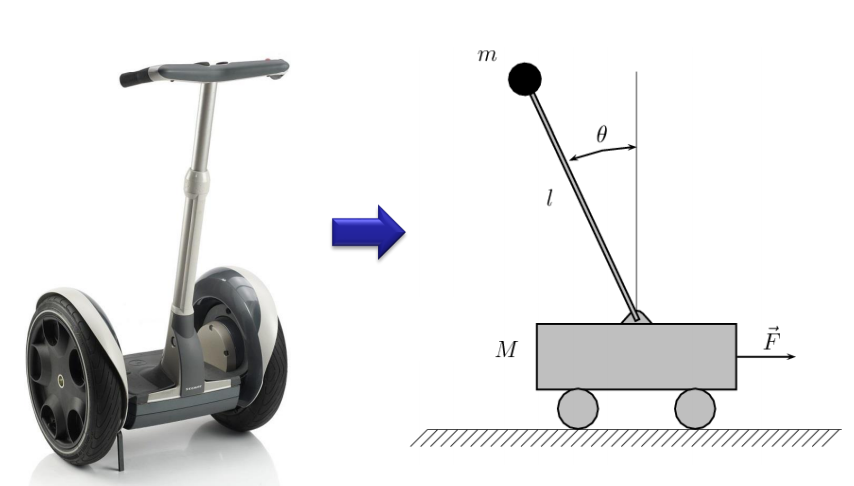
\includegraphics[scale=0.6]{portada.png}
\end{figure}

\hspace{2cm}

\hspace{1cm}
\begin{tabular}{|c| p{122mm}|}
	\hline
	\multirow{4}{50mm}{\\ \centering \large Apellidos y nombres}	 &  \\  
	& Alfaro Domínguez Rodrigo  \\  \cline{2-2}
	&  \\  
	& Barrera Peña Víctor Miguel \\  \cline{2-2}
	&  \\  
	& Villeda Hernández Erick Ricardo \\ 
	\hline
\end{tabular}
\begin{tabular}{|p{50mm} | c | p{80mm}| p{23mm} |}
	Grpo: & 4 & \multirow{2}{90mm}{Profesor: M.I Lauro Fernando Vazquez Alberto } & Calificación \\ \cline{1-2}
	Brigada: & 1 &  &\\ \hline
	Semestre: & 2021-1 & Fecha de ejecución: 24/11/2020 & \\ \hline
\end{tabular}





	\noindent \justifying
\section{Previo}


\subsection{Identificar 2 sistemas físicos que se tengan en casa, con almacenadores de flujo y esfuerzo}


`` \textbf{Almacenadores de energía:} Existen dos tipos: (a) almacenadores de esfuerzo (almacenadores de potencial) y (b) almacenadores de flujo
(almacenadores cinéticos) ''\cite{w1}.

''\textbf{Los almacenadores cinéticos} se caracterizan por leyes constitutivas (o
estado) que relacionan el flujo y el momento (cantidad de movimientos),
esto es f (p) o p(f )''\cite{w1}.


''\textbf{Los almacenadores de potencial} se caracterizan por leyes
constitutivas que relacionan el esfuerzo y el desplazamiento, esto es e(q)
o q(e)''\cite{w1}.\\

Recuerdo que en un libro de Katsuhiko Ogata decía que nosotros como ingenieros modelamos sistemas a partir de modelos que ya tenemos intentando realizar un fenómeno al contrario de los investigadores en ciencias que modelan intentado aproximar un fenómeno natural. En resumidas cuentas nosotros pasamos de la teoría a la practica y los investigadores de ciencia al revés.

El anterior parrafo toma mucho sentido al intentar pasar de las siguientes leyes a sistemas físicos.

\begin{figure}[H]
	\centering
	\caption{Leyes constitutivas de almacenadores cinéticos obtenidas de \cite{w1}}
	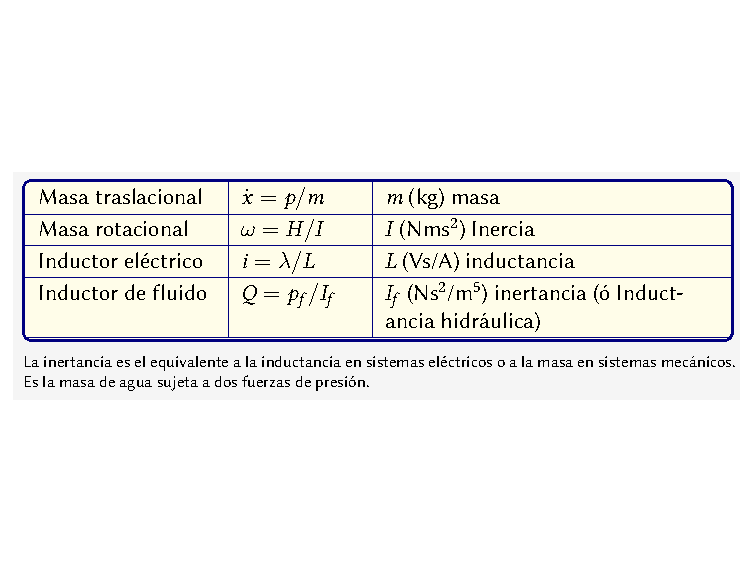
\includegraphics[width=0.7\linewidth]{latex/tabla1}

	\label{fig:tabla1}
\end{figure}

\begin{figure}[H]
	\centering
	\caption{Leyes constitutivas de almacenadores potenciales obtenidas de \cite{w1}}
	\includegraphics[width=0.7\linewidth]{latex/tabla2}
	\label{fig:tabla2}
\end{figure}

\subsubsection{Almacenadores de esfuerzo}

\begin{enumerate}
	\item A partir de \textbf{masa traslacional} deducimos un sistema que mantenga la inercia; algo de lo más apreciable es pensar en una fila de dominós parada, la señal es el simple toque del dedo, ocasionando que vayan cayendo una a una las fichas.
	\item A partir de \textbf{inductor eléctrico} de la figura \ref{fig:tabla1}; deduciendo que un circuito que utilice un inductor por ejemplo en el circuito que lleva en estos momentos la fuente de alimentación de mi computadora, las señales tanto son la corriente que se utiliza para funcionar, como aquella que manda el sistema para solicitar más energía.
\end{enumerate}

\subsubsection{Almacenadores de potencia}

\begin{enumerate}
	\item Usando la idea de \textbf{resorte traslacionar} Pienso en la idea de los resortes de colchón, ya que dentro de la estructura existenten muchos de ellos y si me acuesto, la fuerza aplicada gracias a la gravedad estando en reposo, complementarían la idea de un sistema.
	\item Usando la idea de capacitor eléctrico recurro a la idea mi computadora (de escritorio) tiene varios capacitores donde la entrada es el voltaje ofrecido por la fuente de poder expulsado  hacia los componentes de la computadora. En idea se usan capacitores, se necesitan calcular los voltajes de los componentes y ver el circuito para ver porque fuerón colocaados ahí.
\end{enumerate}

\subsection{¿Qué sistemas con elementos disipadores conoce?}
Primero hay que mencionar que son los disipadores para poder asociar la idea y decir que esos son los disipadores. En este caso muestro una tabla con los disipadores ideales.

\begin{figure}[H]
	\centering
	\caption{Disipadores ideales \cite{w1}}
	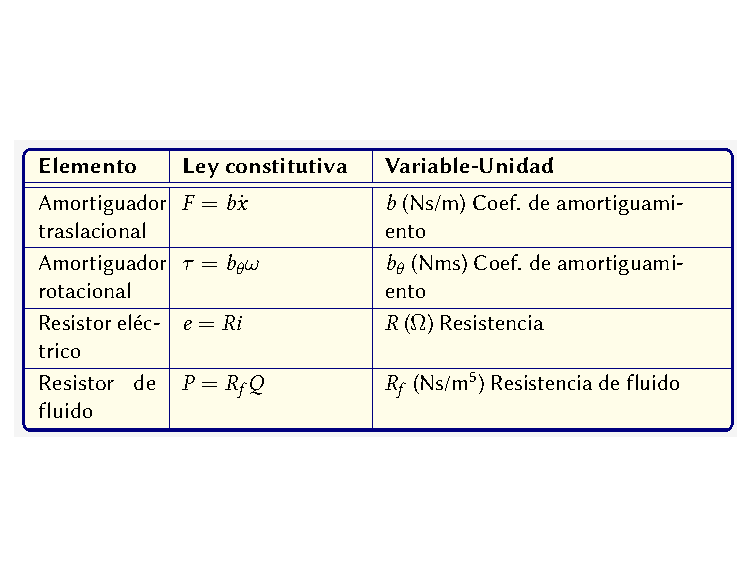
\includegraphics[width=0.7\linewidth]{latex/tabla3}
	\label{fig:tabla3}
\end{figure}

''La disipación de potencia de un disipador ideal por virtud de flujo $ f  $ se
representa por una función de disipación, o contenido $ \mathcal{D}(f) $ definida por

\begin{equation*}
	\mathcal{D}(f):=\int e(f) d f
\end{equation*}	

''\cite{w1}.

El disipador se utiliza en sistemas \textbf{eléctricos, mecánicos traslacionales y mecánicos rotacionales}	. Todos los disipadores se pueden clasificar en dos categorías: activos y pasivos.\\



Existen varias maneras de dividir los disipadores, pero una forma de categorizar al sistema que disipa la energía es diciendo como funciona dicho sistema, si este disipa por un medio de control. Si este control es nulo y no necesitas programarlo para que realice una acción este será pasivo.

Si el sistema de disipación necesita que se active cierto control entonces este será activo, aunque también existen otras combinaciones como hibrido, semiactivo. Estos dos últimos tipos dependen del elemento, en el caso de amortiguadores si existe, de caso de fluido lo desconozco, y en el caso de energía calorífica existe; hablando de este último tipo de sistemas mostraré unos ejemplos viniendo de sistemas que como ingenieros en computación veremos a diario:

\paragraph{Disipadores activos}

Estos suelen tener un ventilador de alguna clase, siendo los de rodamientos y motor los más comunes. Su rendimiento es excelente, pero son más bien caros al tener partes móviles.\

\paragraph{Disipadores pasivos}
Estos no tienen componentes mecánicos, y emplean solo la convección para disipar la energía térmica. Al no tener partes móviles, son más fiables, pero es necesario que el aire circule por las aletas.

\textbf{Algunos sistemas con elementos disipadores son:}

\begin{itemize}
	\item Se emplea sobre transistores en circuitos electrónicos de potencia para evitar que las altas temperaturas puedan llegar a quemarlos.
	\item En las computadoras su uso es intensivo y prolongado, ya que sirve para que algunas tarjetas gráficas o el microprocesador puedan disminuir sus altas temperaturas.
	\item Otro sistema en donde se utilizan los disipadores son en las consolas de videojuegos.
\end{itemize}

\paragraph{Recordar}

Hay dos puntos que siempre tenerlos en la mente mencionados en \cite{w1} y que los tomo literalmente del texto:

\begin{itemize}
	\item Los puertos son los puntos de interconexión entre elementos y
	subsistemas.
	\item La fuentes de energía, los almacenadores y los disipadores son
	elementos de un puerto, transformadores de potencia y transductores
	son elementos con dos puertos.
	\item Disipadores de energía: Sólo existe un tipo: disipador de energía
	generalizado.

\end{itemize}

Usted dirá con respecto al punto 3 ¿Pero si por qué dice que no existe tipos, si me mostró anteriormente que hay pasivos, activos, etc? Yo dije categorización o conjunto, pero no sobre los disipadores, sino sobre el mecanismo que lograba llevar a cambo el disipador, es decir, ya a su aplicación. En disipadores no existen tipos, pero en el mecanismo de disipación, existe.
	
\subsection{¿Cuáles son las fuentes de esfuerzos y flujos en sistemas eléctricos y mecánicos?}

Veamos la fuentes de energía tomando como cita textual lo dicho del medio \cite{w1}\\

\textbf{Fuentes de energía:} Dos tipos de fuentes de energía generalizadas
existen: 
\begin{itemize}
	\item (a) fuentes de esfuerzo
	\item (b) fuentes de flujo.
\end{itemize}

\begin{figure}[H]
	\centering
	\caption{Fuentes de energía \cite{w1}}
	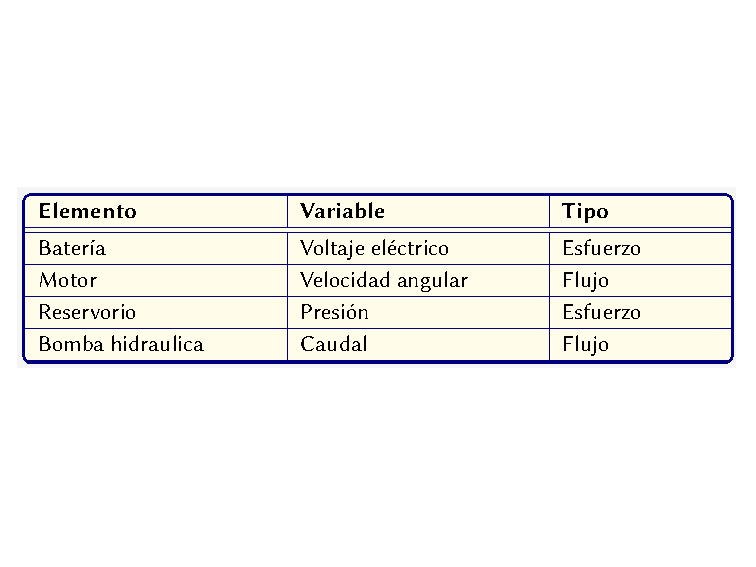
\includegraphics[width=0.7\linewidth]{latex/tabla5}
	\label{fig:tabla5}
\end{figure}


Esa la tabla mostrada es una pero no muestra las formulas para determinarlas, por ello recurrimos a una siguiente cita textual y a una tabla que lo contiene, además que esta cita si te dice para cual es la conexión con las fuentes de energía.

"Los sistemas físicos se caracterizan por el intercambio de energía entre subsistemas. El lenguaje gráfico Bond Graph es una herramienta para obtener modelos matemáticos a partir de dicho intercambio, representando de manera unificada el flujo de potencia instantánea, los fenómenos de transformación, almacenamiento y disipación de energía y las relaciones estructurales.” \cite{w2}.

Una de las variables que describen los sistemas Bond Graph es el flujo de potencia entre sistemas y subsistemas. Dicha variable está a su vez compuesta por el esfuerzo (e) y el flujo (f), siendo la potencia el producto de ambas variables. Ambas variables son denominadas variables generalizadas de potencia y dependiendo del dominio físico de estudio es que van a representar. En la siguiente tabla podemos ver que representan el esfuerzo y el flujo dependiendo de los sistemas físicos analizados.

\begin{figure}[H]
	\centering
	\caption{Fuentes de energía con sus formulas}
	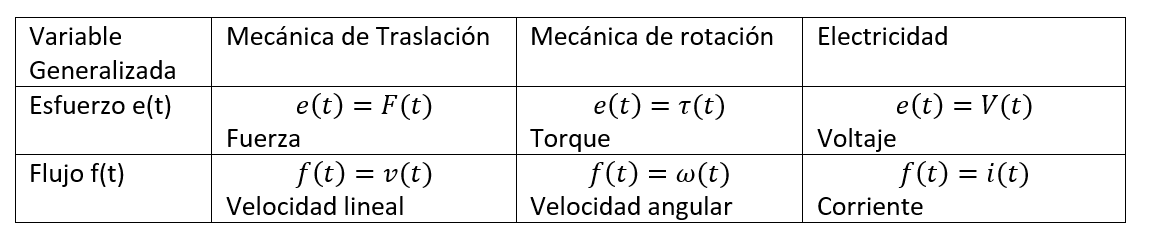
\includegraphics[width=0.7\linewidth]{img/tabla4}
	\label{fig:tabla4}
\end{figure}


\subsection{Traer un elemento físico (mecánico o eléctrico) para su análisis.}

\begin{figure}[H]
	\centering
	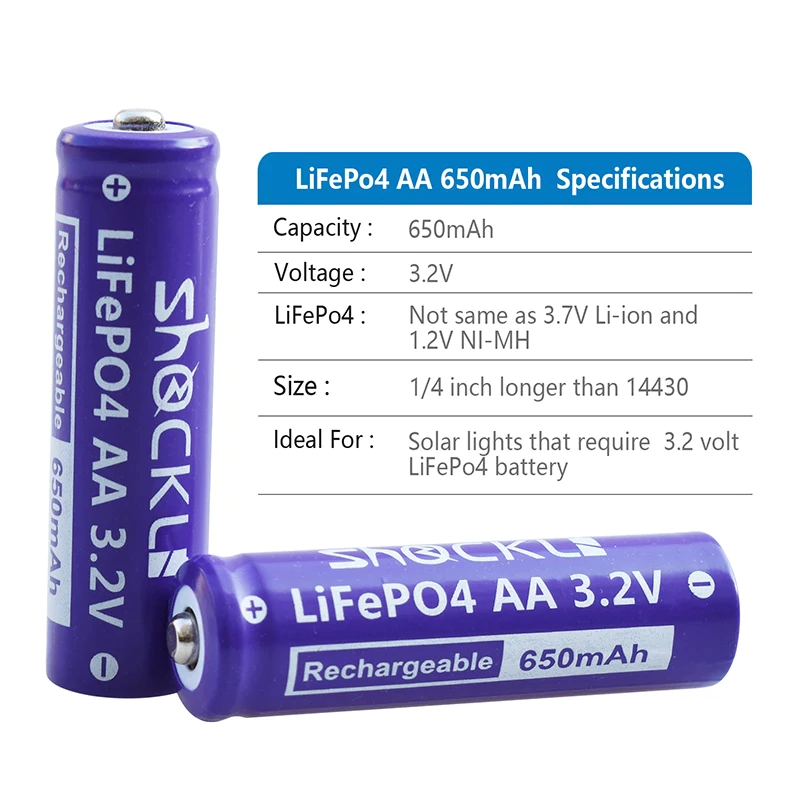
\includegraphics[width=0.5\linewidth]{img/Pila}
	\caption{Pila}
	\label{fig:pila}
\end{figure}



	%\cite{webNijtEdu}\cite{cnxOpenStax} g
	\nocite{*}
	\bibliographystyle{plain}
	\bibliography{latex/previo4.bib}
	\subsection{Sitios de interés}
	
	Te preguntarás que son estos sitios asociados, la respuesta es curiosa, durante la invesigación se encontro material que no se incluyó en este documento, ya que carercia de relevancia para las preguntas, pero de hecho ayudaba si gustabas profundizar, los videos son para dar ilustraciones de sistemas de amortiguamiento, el (7) es acerca de un temario de sistemas dinámicos (en caso de quieras guiarte a estudiarlos).
	
	El (9) es una tesís donde vienen incluida definicones de sistemas dinámicos y su empleo, (10) apuntes sobre sistemas dinámicos, (11) son apuntes de sistemas dinámicos hechos por una investigadora, en lo personal profundiza para nivel de una maestría, irrelevante para nuestro caso, pero puede llegar a ser útil.
	
	\begin{enumerate}
		\item \url{https://www.fceia.unr.edu.ar/control/ssc/}
		\item \url{https://revistas.unal.edu.co/index.php/dyna/article/download/1742/11580}
		\item \url{https://www.youtube.com/watch?v=MO4pXone5Eg&vl=es}
		\item \url{http://www.juntadeandalucia.es/averroes/centros-tic/21700290/helvia/aula/archivos/repositorio/0/41/html/acumul.html}
		\item \url{https://sites.google.com/site/mecanismosmarcos/10-elementos-auxiliares-de-maquinas/3-disipadores-de-energia-mecanica}
		\item \url{https://www.youtube.com/watch?v=W0nJZRmjGVA}
		\item \url{https://www.youtube.com/watch?v=mWCmVoB5EtE}
		\item \url{http://cms.dm.uba.ar/depto/public/fasc5.pdf}
		\url{https://www.cuautitlan.unam.mx/licenciaturas/tecnologia/descargas/DINAMICA_DE_SISTEMAS_FISICOS.pdf}
		\item \url{http://www.ptolomeo.unam.mx:8080/xmlui/bitstream/handle/132.248.52.100/8780/tesis.pdf?sequence=1}
		\item \url{https://www.uv.es/vbolos/docencia/mplmd/apuntes.pdf}
		\item \url{https://www.lizeth-torres.info/curso-din%C3%A1mica-de-sistemas-f%C3%ADsicos/}
	\end{enumerate}
\end{document}

